\chapter{Resultados}\label{cap:pru}

Este capítulo presenta los resultados del trabajo siguiendo el orden del proceso experimental. En primer lugar, se analiza el entrenamiento del agente base y la selección del \textit{checkpoint} que se utiliza como punto de partida de la compresión (Secciones~\ref{sec:res_entrenamiento} y~\ref{sec:res_seleccion}). A continuación, se presentan los resultados de cada técnica de compresión sobre las topologías de entrenamiento, que sirvieron para fijar su configuración (Sección~\ref{sec:res_compresion}), y el tamaño y la latencia de los modelos resultantes (Sección~\ref{sec:res_coste}). La evaluación principal, sobre tres topologías no utilizadas en ninguna fase anterior, se recoge en la Sección~\ref{sec:res_calidad}, y la Sección~\ref{sec:res_mayores} la extiende a siete redes de mayor tamaño. La Sección~\ref{sec:res_energia} analiza el tiempo de optimización y su impacto energético, y la Sección~\ref{sec:res_milp} compara ENERO, original y comprimido, con la formulación exacta del mismo problema. Por último, la Sección~\ref{sec:res_sintesis} resume la aportación de cada técnica, su idoneidad según el tipo de red y la metodología más adecuada para este problema.

% =====================================================================
\section{Entrenamiento del agente base}\label{sec:res_entrenamiento}

Al final de cada episodio de entrenamiento (una iteración de PPO: recogida de 835 transiciones y actualización de la política, Sección~\ref{sec:hiperparametros_base}), el agente se evalúa con su política determinista sobre las 60 matrices de validación (las matrices 0 a 19 de la partición \texttt{EVALUATE} de BtAsiaPac, Garr199905 y Goodnet; Sección~\ref{sec:datos}). En cada matriz se calculan el retorno del episodio $G$ (Ecuación~\eqref{eq:retorno_v17}) y la MLU de la configuración final (Ecuación~\eqref{eq:mlu}), y las figuras de esta sección representan la media de ambas métricas sobre las 60 matrices. Como estos valores oscilan mucho de un episodio a otro, se representa también su media móvil, es decir, el promedio de los 10 últimos episodios, que suaviza las oscilaciones y permite apreciar la tendencia.

Estas métricas sirven para seguir el aprendizaje del agente; el coste de usarlo una vez entrenado, que es el que interesa en operación, se analiza en las Secciones~\ref{sec:res_coste} y~\ref{sec:res_energia}.

\subsection{Evolución del retorno}\label{sec:res_recompensa}

Cada optimización de una matriz de tráfico parte de la configuración de OSPF, y el retorno $G$ compara con ella la configuración en la que termina el agente (Ecuación~\eqref{eq:retorno_v17}): un valor positivo indica que la configuración final mejora a OSPF, un valor nulo que la iguala y uno negativo que la empeora. Es una magnitud adimensional, porque tanto la MLU como la desviación típica de las utilizaciones son cocientes entre carga y capacidad. Por ejemplo, un retorno de $+1$ equivale a reducir en $0{,}1$ la suma de ambas, es decir, en diez puntos porcentuales de utilización. Conviene distinguir este retorno de la solución que entrega ENERO: el sistema conserva la mejor configuración encontrada durante la optimización, que nunca es peor que la de OSPF (Sección~\ref{sec:enero}), mientras que el retorno mide dónde termina la política. La Figura~\ref{fig:ent_recompensa} muestra su evolución a lo largo del entrenamiento.

\begin{figure}[H]
	\centering
	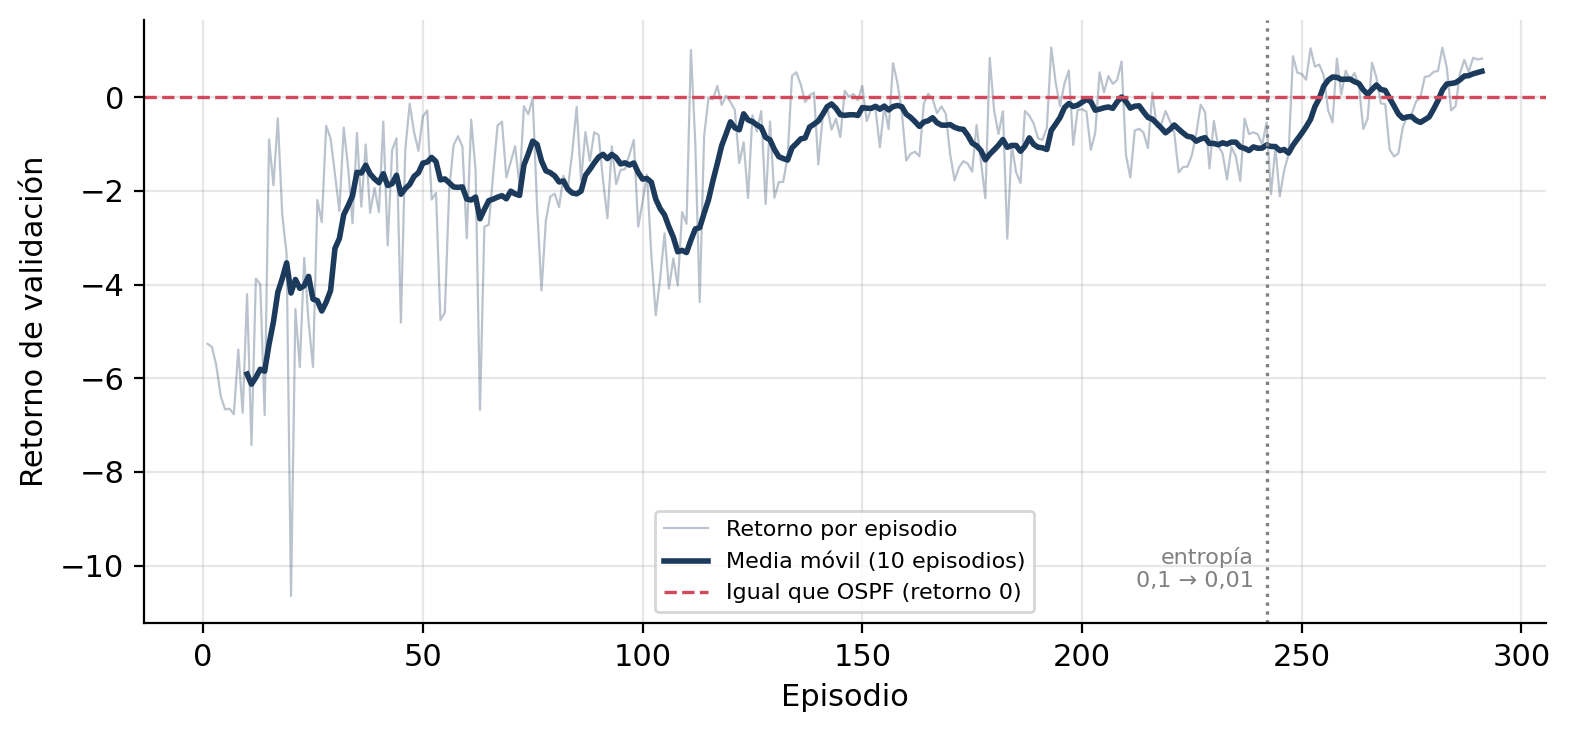
\includegraphics[width=\textwidth]{imagenes/fig_ent_recompensa}
	\caption[Retorno de validación durante el entrenamiento]{Retorno de validación por episodio y su media móvil de 10 episodios. La línea discontinua marca el retorno nulo, que equivale a igualar a OSPF, y la vertical punteada, la reducción del coeficiente de entropía $c_2$ en el episodio 242. El retorno es adimensional y el eje horizontal indica episodios de entrenamiento (iteraciones de PPO).}
	\label{fig:ent_recompensa}
\end{figure}

Al principio del entrenamiento, el retorno medio es de $-5{,}3$: un agente sin entrenar elige caminos casi al azar y termina en configuraciones peores que la de OSPF. A medida que aprende, el retorno crece, y en los mejores episodios supera el cero, con un máximo de $+1{,}06$. Es decir, el número de episodios de entrenamiento no indica cuánto tarda una optimización, sino cuánto tarda el agente en aprender una política cuya configuración final mejora a OSPF de forma consistente; esto solo ocurre en la mayoría de los episodios tras reducir el coeficiente de entropía $c_2$ de la función de pérdida de PPO (Ecuación~\eqref{eq:ppo_loss}), como se analiza en la Sección~\ref{sec:res_entropia}. Además, el retorno y la MLU media de validación están casi perfectamente relacionados (coeficiente de correlación $r = -0{,}998$): los episodios con mayor retorno son, casi sin excepción, los de menor MLU. El término de dispersión añadido no desvía, por tanto, al agente de su objetivo principal, y el retorno es un buen criterio para elegir el modelo.

\subsection{Calidad del enrutamiento durante el entrenamiento}\label{sec:res_mlu_entrenamiento}

La Figura~\ref{fig:ent_mlu} muestra la MLU de validación al final de cada episodio: la media de las 60 matrices y la de la peor de ellas, es decir, la que tiene la MLU más alta en ese episodio.

\begin{figure}[H]
	\centering
	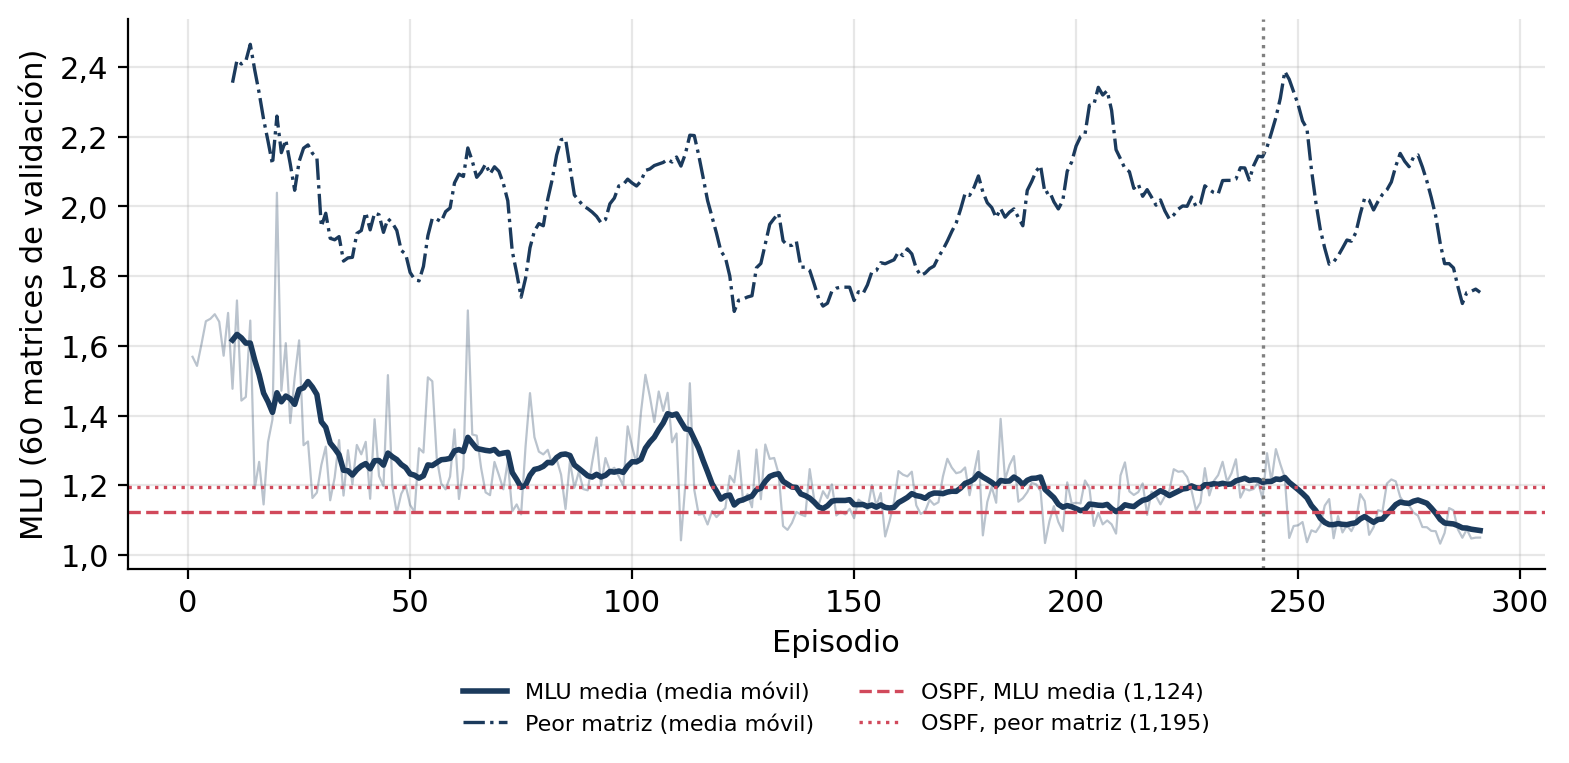
\includegraphics[width=\textwidth]{imagenes/fig_ent_mlu}
	\caption[MLU de validación durante el entrenamiento]{MLU de validación durante el entrenamiento: media de las 60 matrices de validación y MLU de la peor matriz en cada episodio, con su media móvil de 10 episodios, frente a los valores de OSPF (1,124 y 1,195). La MLU es adimensional (carga entre capacidad). La línea vertical marca la reducción del coeficiente de entropía $c_2$.}
	\label{fig:ent_mlu}
\end{figure}

Con OSPF, la MLU media de validación es de 1,124: en promedio, el enlace más cargado recibe un 12\,\% más de tráfico que su capacidad (Sección~\ref{sec:datos}). El agente baja de ese valor a lo largo del entrenamiento, hasta alcanzar 1,033 en el episodio 282, un 8,1\,\% menos. También reduce la dispersión de la carga, de 0,219 con OSPF a unos 0,20, de modo que la MLU no se reduce a costa de desequilibrar el resto de la red.

El comportamiento en el peor caso es distinto. La curva superior de la figura representa, en cada episodio, la MLU de la matriz de validación con mayor MLU al final del episodio, que no es siempre la misma, ya que depende de las decisiones del agente en cada momento. Esta MLU se mantiene por encima de la del peor caso de OSPF (1,195) durante todo el entrenamiento. Es decir, un agente que mejora a OSPF en media puede empeorarlo en matrices concretas. Por este motivo, ENERO conserva siempre la mejor configuración encontrada durante la optimización, que como mínimo es la de OSPF, y la refina después con la LS.

\subsection{Efecto de la reducción de la entropía}\label{sec:res_entropia}

Durante el entrenamiento, la función de pérdida de PPO incluye un término que premia la entropía de la política, es decir, de la distribución de probabilidad que el actor asigna a los nodos intermedios candidatos en cada decisión, ponderado por el coeficiente $c_2$ (Ecuación~\eqref{eq:ppo_loss}). Una entropía alta significa que las probabilidades están repartidas entre muchos candidatos, lo que favorece la exploración; una entropía baja, que el agente concentra la probabilidad en pocos de ellos. La Tabla~\ref{tab:res_entropia} compara el retorno de validación antes y después de reducir $c_2$ de 0,1 a 0,01 en el episodio 242.
\begin{table}[H]
	\centering
	\footnotesize
	\begin{adjustbox}{max width=\textwidth}
	\begin{tabular}{lccc}
		\toprule
		\textbf{Tramo} & \textbf{Episodios} & \textbf{Retorno medio} & \textbf{Episodios con retorno $> 0$} \\
		\midrule
		Entropía $c_2 = 0{,}1$ (últimos 100) & 143--242 & $-0{,}64$ & 19 de 100 (19\,\%) \\
		Entropía $c_2 = 0{,}01$ & 243--291 & $+0{,}02$ & 28 de 49 (57\,\%) \\
		Últimos 10 episodios & 282--291 & $+0{,}55$ & 8 de 10 (80\,\%) \\
		\bottomrule
	\end{tabular}
	\end{adjustbox}
	\caption{Retorno de validación antes y después de reducir el coeficiente de entropía $c_2$ de la política.}
	\label{tab:res_entropia}
\end{table}

Con $c_2 = 0{,}1$, la configuración final del agente mejoraba a OSPF solo en episodios aislados; tras reducir $c_2$, lo hace en la mayoría. Premiar la entropía favorece la exploración, pero introduce aleatoriedad en la política; al reducir su peso, el agente consolida las acciones que mejor funcionan y su comportamiento se vuelve más estable. El mejor retorno, en cambio, apenas cambia: 1,056 en el episodio 282 frente a 1,063 en el 193.

% =====================================================================
\section{Selección del modelo base}\label{sec:res_seleccion}

El episodio 193 obtuvo el mayor retorno de validación de todo el entrenamiento. Sin embargo, en ese momento no era posible saber si el agente seguiría mejorando: el retorno oscila mucho de un episodio a otro y el coeficiente de entropía seguía siendo alto, de modo que la política aún no se había consolidado. Por ello se continuó el entrenamiento, guardando un \textit{checkpoint} en cada episodio, y el modelo se eligió al final comparando los mejores candidatos con datos que no se habían utilizado para seguir el entrenamiento.

Los candidatos fueron el 193, el de mayor retorno antes de reducir la entropía; el 282, con el mayor retorno después de la reducción y la mejor MLU media de todo el entrenamiento; y el 252, otro buen candidato de la fase de entropía baja. Se compararon sobre las matrices 20 a 49 de la partición \texttt{EVALUATE} de las topologías de entrenamiento, que no se habían usado en la validación (que emplea las matrices 0 a 19). La Tabla~\ref{tab:res_seleccion} recoge la mejora sobre OSPF de la etapa DRL con dos criterios: la mejor configuración del episodio, que es la que ENERO conserva, y la configuración al final del episodio.

\begin{table}[H]
	\centering
	\footnotesize
	\begin{adjustbox}{max width=\textwidth}
	\begin{tabular}{lcccc}
		\toprule
		\textbf{Checkpoint} & \textbf{BtAsiaPac} & \textbf{Garr199905} & \textbf{Goodnet} & \textbf{Media} \\
		\midrule
		\multicolumn{5}{l}{\textit{Mejor configuración del episodio}} \\
		193 & 41,1\,\% & 5,1\,\% & 9,6\,\% & 18,6\,\% \\
		282 & 40,4\,\% & 3,9\,\% & 11,6\,\% & 18,6\,\% \\
		252 & 39,7\,\% & 6,1\,\% & 10,4\,\% & 18,8\,\% \\
		\midrule
		\multicolumn{5}{l}{\textit{Configuración al final del episodio}} \\
		193 & 41,0\,\% & $-16{,}6$\,\% & $-2{,}7$\,\% & 7,2\,\% \\
		282 & 36,7\,\% & $-10{,}4$\,\% & $+1{,}4$\,\% & 9,2\,\% \\
		252 & 38,5\,\% & $-15{,}7$\,\% & $-1{,}9$\,\% & 7,0\,\% \\
		\bottomrule
	\end{tabular}
	\end{adjustbox}
	\caption[Mejora sobre OSPF de los checkpoints candidatos]{Mejora de la MLU sobre OSPF de la etapa DRL de los \textit{checkpoints} candidatos, en las matrices 20 a 49 de \texttt{EVALUATE} de las topologías de entrenamiento. Cada \textit{checkpoint} es un modelo ya entrenado que se evalúa sin seguir aprendiendo.}
	\label{tab:res_seleccion}
\end{table}

Con la mejor configuración del episodio, los tres candidatos son prácticamente iguales. La diferencia aparece al final del episodio: el 282 es el que menos empeora y el único que termina por encima de OSPF en Goodnet. Por esa mayor robustez, por tener la mejor MLU media y por proceder de la fase estable del entrenamiento, se eligió el \textit{checkpoint} 282 como modelo base. La comparación deja además dos observaciones útiles:

\begin{itemize}
	\item \textbf{Conservar la mejor configuración es esencial}. En Garr199905, los tres candidatos terminan el episodio peor que OSPF, mientras que su mejor configuración lo mejora: la política acierta en las primeras demandas y deshace después parte de lo conseguido. Este comportamiento es coherente con el factor de descuento $\gamma = 0{,}95$ (Ecuación~\eqref{eq:retorno}), con el que las recompensas del final de un episodio largo tienen poco peso (Sección~\ref{sec:analisis_recompensa}), y justifica el diseño de ENERO.
	\item \textbf{Políticas distintas pueden rendir igual}. Los \textit{checkpoints} 282 y 193 eligen el mismo nodo intermedio en solo el 20--26\,\% de las decisiones en BtAsiaPac y Garr199905, y, sin embargo, obtienen mejoras casi idénticas. Existen muchas formas de desviar el tráfico con resultados muy similares.
\end{itemize}

Conviene distinguir aquí dos costes. El entrenamiento, de unas 87 horas, se realiza una sola vez, con las tres topologías de entrenamiento a la vez (Sección~\ref{sec:hiperparametros_base}), y antes de desplegar el agente, del mismo modo que se diseña cualquier otro sistema antes de ponerlo en servicio. No hay que repetirlo para cada topología: el agente entrenado se aplica directamente, sin volver a entrenar, a cualquier matriz de tráfico y a topologías que no ha visto, como las de las Secciones~\ref{sec:res_calidad} y~\ref{sec:res_mayores}. Los resultados de la Tabla~\ref{tab:res_seleccion} corresponden a esos modelos ya entrenados, que optimizan cada matriz de tráfico nueva sin volver a aprender: en las redes de este tamaño, la etapa DRL tarda unos pocos segundos por matriz y la optimización completa con la LS, del orden de 10 a 20 segundos (Sección~\ref{sec:res_energia}). Esa rapidez en operación es la ventaja que persigue ENERO frente a los métodos clásicos: OSPF no necesita un optimizador centralizado, porque cada enrutador calcula sus caminos de forma distribuida, aunque a cambio de recursos de la red (intercambio de mensajes de estado de enlace) y de un retardo de convergencia; pero no tiene en cuenta la carga y deja una MLU considerablemente peor, y la formulación exacta del enrutamiento por punto intermedio es un problema de programación entera NP-hard, cuyo tiempo de resolución puede crecer rápidamente con el tamaño de la red (Sección~\ref{sec:prog_mat}). La Sección~\ref{sec:res_milp} comprueba si esa ventaja se cumple en las redes evaluadas.

% =====================================================================
\section{Resultados de la compresión en validación}\label{sec:res_compresion}

Esta sección presenta el resultado de cada técnica de compresión durante su propio proceso. Todas las cifras son mejoras de la MLU sobre OSPF de la etapa DRL (Ecuación~\eqref{eq:mejora_ospf}), medidas en las matrices de validación de las topologías de entrenamiento (Sección~\ref{sec:datos}). Con estas matrices, el modelo base obtiene una mejora del 18,1\,\%, que es la referencia de esta sección; la cifra difiere ligeramente del 18,6\,\% de la Tabla~\ref{tab:res_seleccion} porque esta se calculó sobre otras matrices. Estos resultados sirvieron para fijar la configuración de cada técnica; la evaluación definitiva, en topologías no vistas, se presenta en la Sección~\ref{sec:res_calidad}.

\subsection{Poda}\label{sec:res_poda}

La Figura~\ref{fig:poda_barrido} muestra la mejora sobre OSPF del modelo base podado a distintos niveles, sin reentrenar, y la que se obtiene al reentrenar con PPO los niveles del 50 y del 90\,\%. El eje horizontal indica el porcentaje de parámetros del actor que valen cero; como los sesgos y la normalización de capa no se podan, podar el 50\,\% de cada matriz equivale a un 48,4\,\% del total de parámetros, y podar el 90\,\%, a un 87,1\,\%.

\begin{figure}[H]
	\centering
	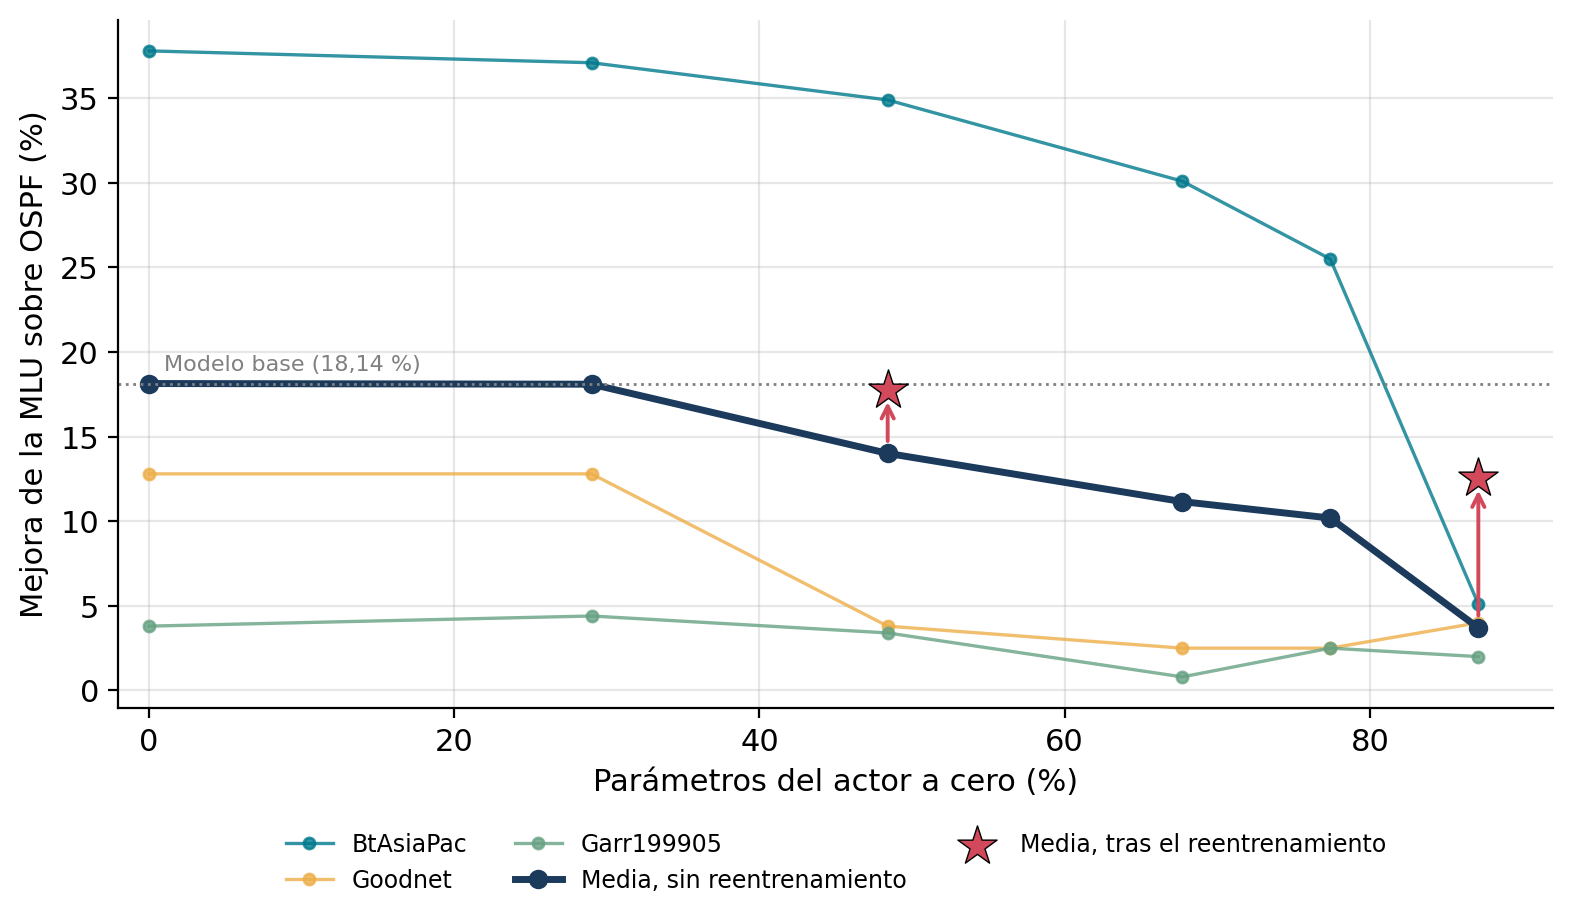
\includegraphics[width=0.95\textwidth]{imagenes/fig_poda_barrido}
	\caption[Mejora sobre OSPF en función del nivel de poda]{Mejora de la MLU sobre OSPF de la etapa DRL en las matrices de validación, en función del porcentaje de parámetros del actor a cero, por topología y en media, sin reentrenamiento. Las estrellas indican la media tras reentrenar los modelos podados al 50 y al 90\,\%.}
	\label{fig:poda_barrido}
\end{figure}

El modelo tiene una redundancia considerable: con un 29\,\% de los parámetros a cero conserva prácticamente toda la mejora del modelo base (18,1\,\%) sin reentrenar. A partir de ese nivel, la calidad disminuye, con un ritmo que depende de la topología. El reentrenamiento recupera la mayor parte de la pérdida: al 50\,\%, la mejora pasa del 14,0 al 17,8\,\%, el 98\,\% de la del modelo base; al 90\,\%, con solo el 13\,\% de los parámetros, pasa del 3,7 al 12,6\,\%, dos tercios de la del modelo base.

\subsection{Cuantización}\label{sec:res_cuantizacion}

La cuantización no requiere reentrenar, por lo que antes de la evaluación completa se comprobó su fidelidad, es decir, cuánto se parecen sus salidas a las del modelo original. Para ello se utilizaron 120 estados obtenidos con matrices de entrenamiento (Sección~\ref{sec:flujo_cuantizacion}) y se midieron dos indicadores: el error absoluto medio de los \textit{logits}, que son las puntuaciones que el actor asigna a cada candidato antes de convertirlas en probabilidades, y el porcentaje de estados en los que el modelo cuantizado elige el mismo candidato que el original. La Tabla~\ref{tab:res_cuantizacion} recoge ambos indicadores junto con el tamaño de cada fichero.

\begin{table}[H]
	\centering
	\footnotesize
	\begin{adjustbox}{max width=\textwidth}
	\begin{tabular}{lcccc}
		\toprule
		\textbf{Variante} & \textbf{Tamaño} & \textbf{Frente a TFLite FP32} & \textbf{Error medio en \textit{logits}} & \textbf{Decisiones iguales} \\
		\midrule
		TFLite FP32 (ref.) & 133,5~KB & -- & 0,00002 & 100\,\% \\
		FP16 & 100,7~KB & $-24{,}6$\,\% & 0,054 & 100\,\% \\
		INT8 dinámico & 80,1~KB & $-40{,}0$\,\% & 2,83 & 76,7\,\% \\
		\bottomrule
	\end{tabular}
	\end{adjustbox}
	\caption[Tamaño y fidelidad de las variantes cuantizadas]{Tamaño y fidelidad de las variantes cuantizadas frente al modelo original, en 120 estados de las topologías de entrenamiento. Los \textit{logits} son adimensionales.}
	\label{tab:res_cuantizacion}
\end{table}

La conversión a TensorFlow Lite no altera el modelo: la variante TFLite FP32, que no está cuantizada, toma las mismas decisiones que el original con un error despreciable, de modo que cualquier diferencia de las otras variantes se debe a la cuantización. FP16 conserva todas las decisiones, mientras que INT8 dinámico cambia una de cada cuatro, con un error medio en los \textit{logits} unas 50 veces mayor que el de FP16. La explicación más probable está en la arquitectura del actor, que aplica ocho veces seguidas las mismas funciones de mensaje y actualización (Sección~\ref{sec:agente}): el error de redondeo introducido en cada iteración se acumula en las siguientes. Las GNN recurrentes parecen, por tanto, más sensibles a la cuantización que las redes con una sola pasada por cada capa.

En cuanto al tamaño, la reducción es menor de lo que sugiere el número de bits. Los pesos del actor ocupan unos 50~KB en FP32, 25~KB en FP16 y 13~KB en INT8, pero los ficheros solo se reducen 1,3 y 1,7 veces respecto a la referencia. El motivo es que un fichero de TensorFlow Lite contiene, además de los pesos, la descripción del grafo de operaciones, en la que las ocho iteraciones del paso de mensajes aparecen desplegadas, y esa parte no se cuantiza. En un modelo tan pequeño, la estructura ocupa más que los pesos; en modelos mucho mayores, en los que los pesos dominan el tamaño, la reducción sería más próxima a la teórica.

\subsection{Destilación}\label{sec:res_destilacion}

La Tabla~\ref{tab:res_destilacion} compara las tres configuraciones de destilación probadas (Sección~\ref{sec:flujo_destilacion}). Para cada una se indica la mejora sobre OSPF de la etapa DRL del mejor estudiante en validación y su proporción respecto a la del maestro, que es el modelo base.

\begin{table}[H]
	\centering
	\footnotesize
	\begin{adjustbox}{max width=\textwidth}
	\begin{tabular}{lcccc}
		\toprule
		\textbf{Configuración} & \textbf{$\alpha$} & \textbf{$\tau$} & \textbf{Mejora del mejor estudiante} & \textbf{Respecto al maestro} \\
		\midrule
		Inicial & 0,7 (con término MSE) & 2 & 13,46\,\% & 74\,\% \\
		Sin MSE & 1 & 2 & 17,83\,\% & 98\,\% \\
		Sin MSE, $\tau = 4$ & 1 & 4 & 18,24\,\% & 100\,\% \\
		\bottomrule
	\end{tabular}
	\end{adjustbox}
	\caption[Resultados de las configuraciones de destilación]{Mejora de la MLU sobre OSPF de la etapa DRL del mejor estudiante de cada configuración, en las matrices de validación. El maestro obtiene un 18,14\,\%.}
	\label{tab:res_destilacion}
\end{table}

La pérdida de destilación combina dos términos (Ecuación~\eqref{eq:kd_total}). El principal, la divergencia KL, mide cuánto se parecen las distribuciones de probabilidad del maestro y del estudiante sobre los candidatos: solo tiene en cuenta qué candidatos prefiere cada modelo y en qué proporción. El auxiliar es el error cuadrático medio (MSE, \textit{Mean Squared Error}): el promedio de los cuadrados de las diferencias entre los \textit{logits} de ambos modelos, es decir, entre los valores numéricos que asignan a cada candidato antes de convertirlos en probabilidades. El peso $\alpha$ reparte la importancia entre ambos.

Con la configuración inicial, $\alpha = 0{,}7$, la pérdida tomaba valores de cientos y oscilaba sin tendencia, el estudiante coincidía con el maestro en solo el 40--55\,\% de las decisiones y su mejora en validación crecía hasta la época 15 y caía después. La causa era el término MSE. Los \textit{logits} del maestro tienen valores grandes, de modo que sus diferencias al cuadrado dominaban la pérdida y obligaban al estudiante a copiar los valores exactos. Pero para decidir solo importa el orden relativo de los \textit{logits}: sumar la misma constante a todos no cambia la decisión. El estudiante, con la mitad de dimensión, no podía reproducir esos valores, y ese objetivo competía con el de la divergencia KL. Al eliminar el MSE ($\alpha = 1$), el estudiante pasa a conservar el 98\,\% de la mejora del maestro.

La temperatura $\tau$ controla cuánto se suavizan las distribuciones antes de compararlas (Ecuación~\eqref{eq:softmax_temp}). Por ejemplo, con \textit{logits} $(5, 4, 1)$, la \textit{softmax} sin suavizar ($\tau = 1$) da probabilidades $(0{,}72,\ 0{,}27,\ 0{,}01)$, mientras que con $\tau = 4$ da $(0{,}47,\ 0{,}36,\ 0{,}17)$: la opción preferida sigue siendo la misma, pero la distribución suavizada indica que la segunda es casi igual de adecuada y que la tercera no es descartable. El maestro, entrenado al final con un coeficiente de entropía bajo, es muy determinista, y con $\tau = 2$ sus distribuciones siguen concentradas casi por completo en un candidato, de modo que aportan poca información sobre los demás. Con $\tau = 4$, el estudiante recibe esa información adicional sobre qué alternativas considera el maestro casi igual de buenas, y su mejora sube de 17,83 a 18,24\,\%. La diferencia es pequeña y está dentro del margen de variación entre ejecuciones, pero va en el sentido esperado. Con esta configuración, el estudiante iguala al maestro en validación con unas 4,6 veces menos parámetros, y es la que se utiliza en el resto del capítulo.

% =====================================================================
\section{Coste de los modelos comprimidos}\label{sec:res_coste}

A partir de esta sección, todos los resultados corresponden al uso de los modelos ya entrenados. La Tabla~\ref{tab:res_coste} recoge el tamaño de cada modelo y su latencia, medida en las topologías de evaluación como la mediana del tiempo de una decisión, es decir, de una llamada al actor con todos los candidatos de una demanda (Sección~\ref{sec:metricas}).

\begin{table}[H]
	\centering
	\footnotesize
	\begin{adjustbox}{max width=\textwidth}
	\begin{tabular}{lrrrrr}
		\toprule
		& & & \textbf{Pesos} & \textbf{Comprimido} & \textbf{Latencia} \\
		\textbf{Modelo} & \textbf{Parámetros} & \textbf{No nulos} & \textbf{(FP32)} & \textbf{(gzip)} & \textbf{mediana} \\
		\midrule
		Original & 12\,737 & 12\,737 & 49,8~KB & 46,0~KB & 16,1~ms \\
		Podado50 & 12\,737 & 6\,577 & 49,8~KB & 28,3~KB & 16,1~ms \\
		Podado90 & 12\,737 & 1\,647 & 49,8~KB & 10,0~KB & 16,1~ms \\
		Estudiante & 2\,753 & 2\,753 & 10,8~KB & 9,9~KB & 5,1~ms \\
		\midrule
		TFLite FP32 & -- & -- & 133,5~KB & 83,5~KB & 72,3~ms \\
		FP16 & -- & -- & 100,7~KB & 50,5~KB & 72,2~ms \\
		INT8 dinámico & -- & -- & 80,1~KB & 27,7~KB & 121,6~ms \\
		\bottomrule
	\end{tabular}
	\end{adjustbox}
	\caption[Tamaño y latencia de los modelos evaluados]{Tamaño y latencia de los modelos evaluados. Para los modelos de TensorFlow Lite, la columna de pesos indica el tamaño del fichero completo. La latencia es la mediana del tiempo por decisión en las tres topologías de evaluación.}
	\label{tab:res_coste}
\end{table}

La poda reduce a la mitad o a la octava parte los parámetros no nulos, pero no el tamaño de las matrices, que conservan los ceros. Su ganancia aparece al almacenar el modelo comprimido: con \texttt{gzip}, el modelo podado al 50\,\% ocupa un 38\,\% menos que el original y el podado al 90\,\%, un 78\,\% menos. En cambio, no reduce la latencia, porque las operaciones de la red multiplican igualmente las matrices completas, incluidos los ceros (Sección~\ref{sec:poda}).

El estudiante es el único modelo que reduce la latencia: con la mitad de dimensión y la mitad de iteraciones, tarda 5,1~ms por decisión frente a los 16,1~ms del original, 3,2 veces menos. La ganancia es mayor cuanto mayor es la topología, porque el coste de cada decisión crece con el número de enlaces y de candidatos (Sección~\ref{sec:drl_te}).

Las variantes de TensorFlow Lite, en cambio, son entre 4,5 y 7,6 veces más lentas que el original ejecutado con TensorFlow. Se comprobó que la diferencia no se debe al número de hilos de cálculo ni a que el intérprete tenga que adaptarse al tamaño de cada entrada: fijando el mismo número de hilos en ambos formatos y midiendo aparte esa adaptación, la diferencia se mantiene. La causa está en la estructura del modelo convertido: las 8 iteraciones del paso de mensajes se despliegan en unas 300 operaciones elementales, porque la activación SELU, la normalización de capa y la celda GRU se descomponen en multiplicaciones, sumas y selecciones, y el intérprete las ejecuta una a una. INT8 dinámico es el más lento porque, además, en cada capa convierte las activaciones a enteros y las devuelve a coma flotante. En este modelo y en este procesador, la cuantización con TensorFlow Lite no aporta velocidad.

% =====================================================================
\section{Calidad del enrutamiento en topologías no vistas}\label{sec:res_calidad}

Esta sección presenta la evaluación principal: todos los modelos, ya entrenados, optimizan las 50 matrices de evaluación de EliBackbone, HurricaneElectric y Janetbackbone, tres topologías que no se han utilizado en ningún momento del entrenamiento, de la compresión ni de la selección de modelos.

\subsection{Resultados globales}

La Tabla~\ref{tab:res_global} resume los resultados medios sobre las 150 matrices. Para cada modelo se indica la mejora de la MLU sobre OSPF (Ecuación~\eqref{eq:mejora_ospf}) que consigue la etapa DRL y la que consigue ENERO completo, es decir, la etapa DRL seguida de la LS (DRL + LS); la distancia de ENERO completo a la cota LP (Ecuación~\eqref{eq:margen_lp}), que indica cuánto le falta para llegar al mínimo teórico y es mejor cuanto menor; y el tiempo medio que tarda en optimizar una matriz. La Figura~\ref{fig:res_mejora} desglosa la mejora por topología.

\begin{table}[H]
	\centering
	\footnotesize
	\setlength{\tabcolsep}{4pt}
	\begin{adjustbox}{max width=\textwidth}
	\begin{tabular}{lcccc}
		\toprule
		& \multicolumn{2}{c}{\textbf{Mejora sobre OSPF}} & \textbf{Distancia a la} & \textbf{Tiempo} \\
		\textbf{Método} & \textbf{DRL} & \textbf{DRL + LS} & \textbf{cota LP (DRL + LS)} & \textbf{por matriz} \\
		\midrule
		Original & 12,6\,\% & 34,3\,\% & 30,7\,\% & 20,0~s \\
		Podado50 & 16,5\,\% & 35,0\,\% & 29,3\,\% & 19,4~s \\
		Podado90 & 5,5\,\% & 32,6\,\% & 34,0\,\% & 21,5~s \\
		Estudiante (media de 4 semillas) & 14,6\,\% & 34,5\,\% & 30,4\,\% & 14,9~s$^{*}$ \\
		TFLite FP32 & 12,6\,\% & 34,3\,\% & 30,7\,\% & 24,8~s \\
		FP16 & 12,7\,\% & 34,5\,\% & 30,4\,\% & 24,9~s \\
		INT8 dinámico & 11,6\,\% & 34,0\,\% & 31,4\,\% & 28,7~s \\
		\midrule
		LS desde OSPF (sin agente) & -- & 31,2\,\% & 36,7\,\% & 17,0~s \\
		\bottomrule
	\end{tabular}
	\end{adjustbox}
	\caption[Resultados medios en las topologías de evaluación]{Resultados medios sobre las 150 matrices de las tres topologías de evaluación. $^{*}$Tiempo del estudiante de la semilla 9, el único medido sin otras cargas en el equipo.}
	\label{tab:res_global}
\end{table}

\begin{figure}[H]
	\centering
	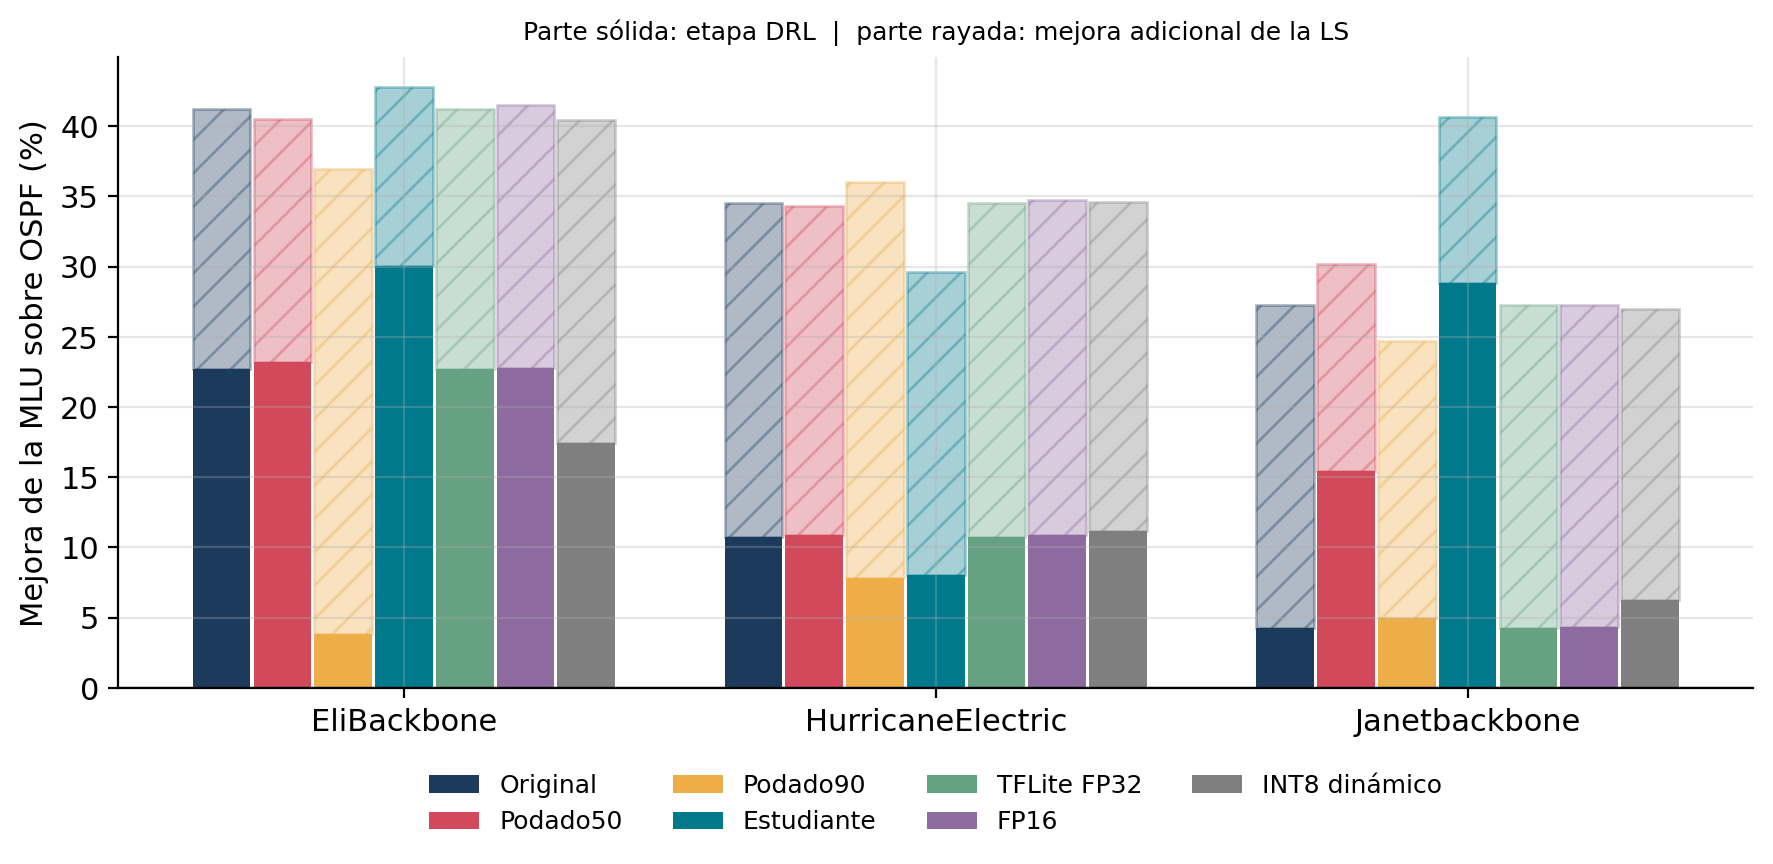
\includegraphics[width=\textwidth]{imagenes/fig_mejora_ospf}
	\caption[Mejora sobre OSPF por topología y modelo]{Mejora media de la MLU sobre OSPF por topología y modelo. La parte sólida de cada barra corresponde a la etapa DRL y la rayada, a lo que añade la LS. El estudiante es el de la semilla 9.}
	\label{fig:res_mejora}
\end{figure}

El resultado principal es que \textbf{la compresión conserva la calidad del enrutamiento}. Con la LS, todos los modelos comprimidos mejoran a OSPF entre un 32,6 y un 35,0\,\% de media, frente al 34,3\,\% del original, y todos superan a la LS aplicada sin agente (31,2\,\%): el agente, comprimido o no, proporciona a la LS un mejor punto de partida.

Para comprobar si las diferencias con el original son reales o se deben a la variabilidad entre matrices, se aplicó la prueba de Wilcoxon a las diferencias de MLU emparejadas por matriz (Sección~\ref{sec:metricas}). El valor $p$ de la prueba es la probabilidad de observar una diferencia al menos tan grande como la medida si ambos modelos fueran igual de buenos; con un valor inferior a 0,05, la diferencia se considera significativa. Para el modelo podado al 50\,\%, FP16 e INT8 dinámico, los valores de $p$ son 0,46, 0,08 y 0,63, de modo que no se observan diferencias estadísticamente significativas entre su calidad y la del original. El modelo podado al 90\,\% es ligeramente peor, con diferencias estadísticamente significativas ($p = 0{,}0008$), aunque la LS compensa casi toda su desventaja en la etapa DRL. La variante TFLite FP32 obtiene exactamente los mismos resultados que el original, lo que confirma la fidelidad de la conversión.\label{sec:res_semillas}

En el caso del estudiante, el primer modelo destilado (semilla 9) obtuvo una mejora del 37,7\,\%, superior a la del original. Para comprobar si ese resultado era estable, la destilación se repitió con otras tres semillas aleatorias, que cambian la inicialización de los pesos del estudiante y el orden en que recibe los datos; no se realizaron más repeticiones porque cada destilación y su evaluación ocupan el equipo varias horas. Los cuatro estudiantes obtienen en validación resultados muy parecidos, entre un 17,0 y un 18,6\,\% de mejora en la etapa DRL, pero en las topologías de evaluación su mejora con LS varía entre el 32,3 y el 37,7\,\%. En media, el estudiante mejora a OSPF un 34,5\,\%, prácticamente lo mismo que el original, y esa es la cifra que figura en la tabla. La destilación conserva, por tanto, la calidad del original reduciendo su latencia 3,2 veces, pero el resultado de un estudiante concreto varía con el entrenamiento, por lo que conviene validarlo en la red en la que se vaya a desplegar.

\subsection{Acuerdo de decisiones}

El acuerdo de decisiones indica en qué porcentaje de las decisiones un modelo comprimido elige el mismo candidato que el original ante el mismo estado (Sección~\ref{sec:metricas}). En las topologías de evaluación es del 99,3\,\% para FP16 y del 53\,\% para INT8 dinámico, pero mucho menor en los modelos cuyos pesos se vuelven a entrenar durante la compresión, siempre con las topologías de entrenamiento y nunca con las de evaluación: del 21\,\% para el podado al 50\,\% y el estudiante, y del 8\,\% para el podado al 90\,\%. A pesar de ello, el podado al 50\,\% no presenta diferencias estadísticamente significativas con el original, el estudiante obtiene en media la misma calidad y el podado al 90\,\% solo es ligeramente peor. Los modelos reentrenados no reproducen las decisiones del original, sino que aprenden su propia política, de calidad similar en media, como ya se vio al comparar los \textit{checkpoints} candidatos (Sección~\ref{sec:res_seleccion}). Por eso un agente comprimido debe evaluarse por la calidad de la tarea completa y no por la fidelidad de sus salidas (Sección~\ref{sec:comp_part}).

\subsection{Generalización y distancia a la cota LP}\label{sec:res_generalizacion}

La etapa DRL del modelo original mejora a OSPF un 12,6\,\% en las topologías de evaluación, frente al 18,6\,\% que obtiene en matrices no utilizadas de las topologías de entrenamiento (Sección~\ref{sec:res_seleccion}). La diferencia se concentra en Janetbackbone, la topología de evaluación más grande, donde la etapa DRL solo mejora a OSPF un 4,3\,\%; aun así, la LS compensa buena parte de la diferencia y ENERO completo mejora a OSPF un 27,3\,\% en esa red. Es la limitación conocida de los agentes entrenados con pocas topologías, que el propio artículo de ENERO señala \cite{ALMASAN2022109166}. En este trabajo se utilizaron las mismas tres topologías de entrenamiento que en el artículo original, porque cada topología adicional alarga el entrenamiento, que en CPU ya requiere cerca de cuatro días. Entre los modelos comprimidos, el único que generaliza claramente peor es el podado al 90\,\%: su etapa DRL conservaba un 12,6\,\% de mejora en validación, pero en las topologías de evaluación se queda en un 5,5\,\%, lo que indica que una poda tan extrema reduce su capacidad de adaptarse a redes nuevas.

La distancia a la cota LP completa este análisis. La cota es la MLU que se obtendría si el tráfico de cada demanda pudiera repartirse libremente entre todos los caminos (Sección~\ref{sec:lp}), algo que ENERO no permite, porque cada demanda sigue un único camino con, como mucho, un nodo intermedio. Es, por tanto, una referencia optimista del margen de mejora, aunque en estas redes resulta ser casi alcanzable: la mejor configuración con un único nodo intermedio por demanda queda a menos de un 0,4\,\% de ella (Sección~\ref{sec:res_milp}). Con el modelo original, ENERO completo queda a un 5\,\% de la cota en EliBackbone, a un 38\,\% en HurricaneElectric y a un 49\,\% en Janetbackbone, siempre más cerca que la LS sin agente (14, 40 y 56\,\%). En la red más pequeña, ENERO se encuentra muy próximo al límite teórico, mientras que en las mayores queda un margen de mejora que podría aprovecharse entrenando con topologías más parecidas a ellas o resolviendo el problema de forma exacta (Sección~\ref{sec:res_milp}).

% =====================================================================
\section{Evaluación en redes mayores}\label{sec:res_escalabilidad}\label{sec:res_tipo_red}\label{sec:res_mayores}

Para comprobar si las conclusiones se mantienen en redes más grandes y distintas de las de entrenamiento, se evaluaron las siete topologías adicionales, de 30 a 43 nodos, con 10 matrices cada una (Sección~\ref{sec:datos}). La Tabla~\ref{tab:res_escal} recoge la mejora sobre OSPF de ENERO completo con cada modelo, junto con la de la LS sin agente y la de la cota LP. Esta última es la mejora máxima teórica, que ningún método puede superar. El grado medio de cada red es el número medio de enlaces por nodo, una medida de la densidad de su estructura; las topologías de evaluación principales tienen un grado medio de 3,0 a 3,1.

\begin{table}[H]
	\centering
	\footnotesize
	\setlength{\tabcolsep}{3.5pt}
	\begin{adjustbox}{max width=\textwidth}
	\begin{tabular}{lcc|ccccc|cc}
		\toprule
		& & \textbf{Grado} & \multicolumn{5}{c|}{\textbf{ENERO completo (DRL + LS)}} & \textbf{LS sin} & \textbf{Cota} \\
		\textbf{Topología} & \textbf{Nodos} & \textbf{medio} & \textbf{Original} & \textbf{Estudiante} & \textbf{Podado50} & \textbf{Podado90} & \textbf{INT8} & \textbf{agente} & \textbf{LP} \\
		\midrule
		WideJpn & 30 & 2,2 & 18,7\,\% & 18,9\,\% & 18,7\,\% & 18,7\,\% & 18,7\,\% & 18,7\,\% & 36,8\,\% \\
		GtsPoland & 33 & 2,2 & 15,7\,\% & 15,0\,\% & 14,9\,\% & 15,2\,\% & 15,6\,\% & 15,0\,\% & 35,2\,\% \\
		Bics & 33 & 2,9 & 25,1\,\% & 24,6\,\% & 26,3\,\% & 21,4\,\% & 22,2\,\% & 16,3\,\% & 29,6\,\% \\
		Evolink & 37 & 2,4 & 9,4\,\% & 9,2\,\% & 9,4\,\% & 9,4\,\% & 9,4\,\% & 9,3\,\% & 16,8\,\% \\
		Cesnet200511 & 39 & 2,3 & 19,9\,\% & 18,8\,\% & 19,3\,\% & 18,1\,\% & 20,9\,\% & 18,0\,\% & 50,3\,\% \\
		LambdaNet & 42 & 2,2 & 11,1\,\% & 10,6\,\% & 11,3\,\% & 9,6\,\% & 10,4\,\% & 10,6\,\% & 17,1\,\% \\
		Sanet & 43 & 2,1 & 13,7\,\% & 14,0\,\% & 12,8\,\% & 13,9\,\% & 13,0\,\% & 14,4\,\% & 15,2\,\% \\
		\midrule
		\textbf{Media} & & & \textbf{16,2\,\%} & \textbf{15,9\,\%} & \textbf{16,1\,\%} & \textbf{15,2\,\%} & \textbf{15,7\,\%} & \textbf{14,6\,\%} & \textbf{28,7\,\%} \\
		\bottomrule
	\end{tabular}
	\end{adjustbox}
	\caption[Resultados en las redes mayores]{Mejora media de la MLU sobre OSPF de ENERO completo (DRL + LS) en las siete redes mayores, con 10 matrices por topología, junto con la de la LS sin agente y la de la cota LP, que es la máxima teórica. El grado medio es el número medio de enlaces por nodo. El estudiante es el de la semilla 9.}
	\label{tab:res_escal}
\end{table}

La primera conclusión es que \textbf{la compresión sigue siendo robusta en redes mayores}. En las 70 matrices, el estudiante y el modelo podado al 50\,\% siguen sin presentar diferencias estadísticamente significativas con el original ($p = 0{,}92$ y $0{,}64$ en la prueba de Wilcoxon), y las diferencias del podado al 90\,\% y de INT8 dinámico son pequeñas, de un punto porcentual o menos de media. Los modelos comprimidos se comportan, por tanto, como el original también fuera de las topologías de evaluación principales.

La Tabla~\ref{tab:res_escal} permite ver también cuánto se acerca ENERO al límite teórico en estas redes. Con el modelo original, obtiene de media el 56\,\% de la mejora máxima posible (16,2 frente a 28,7\,\%), con valores que van desde el 40\,\% de Cesnet200511 hasta el 90\,\% de Sanet. A diferencia de lo observado en las topologías de evaluación principales, en las que la distancia a la cota crece con el tamaño de la red (Sección~\ref{sec:res_generalizacion}), aquí no se aprecia una tendencia clara con el número de nodos: la red más grande, Sanet, es la que queda más cerca de la cota.

La segunda conclusión se refiere al propio agente: \textbf{su aportación depende de lo parecida que sea la red a las de entrenamiento}. En Bics, la única de las nuevas con un grado medio cercano a 3, como las de evaluación y dos de las tres de entrenamiento, ENERO mejora a la LS sin agente en casi 9 puntos porcentuales (25,1 frente a 16,3\,\%). En las otras seis, más dispersas (grado medio de 2,1 a 2,4), la diferencia es pequeña y la mayor parte de la mejora la consigue la LS. La Figura~\ref{fig:res_tipo_red} lo resume para las diez topologías.

\begin{figure}[H]
	\centering
	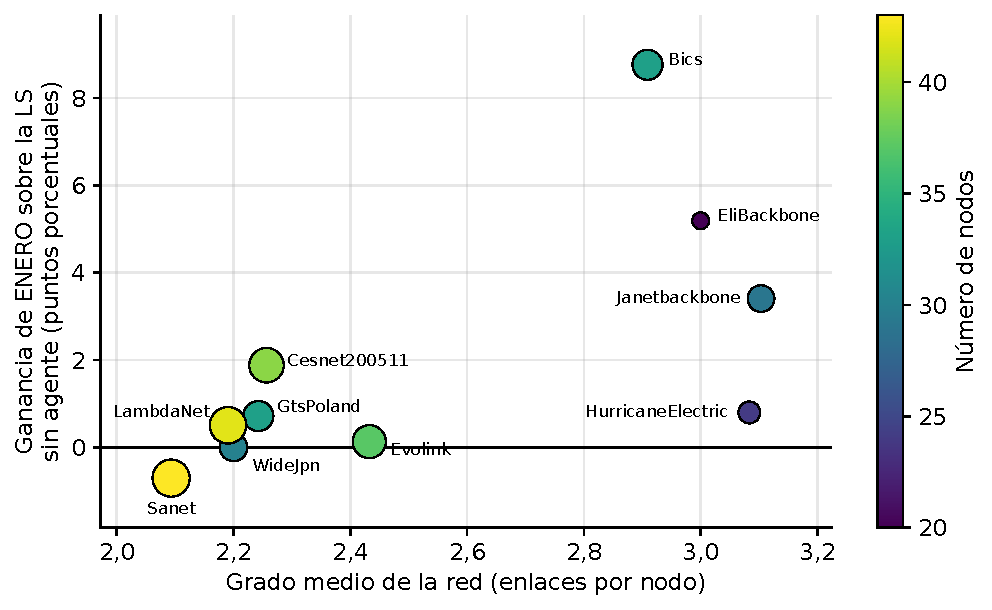
\includegraphics[width=\textwidth]{imagenes/fig_tipo_red}
	\caption[Aportación de ENERO según el grado medio de la red]{Diferencia, en puntos porcentuales, entre la mejora sobre OSPF de ENERO completo (modelo original) y la de la LS sin agente, frente al grado medio de cada topología. Un valor positivo indica que el agente mejora el resultado de la LS. El tamaño y el color de cada punto indican el número de nodos.}
	\label{fig:res_tipo_red}
\end{figure}

El par formado por Bics y GtsPoland, ambas con 33 nodos y con un grado medio de 2,9 y 2,2, respectivamente, indica que lo determinante es la estructura de la red más que su tamaño: en la primera ENERO aporta 8,8 puntos sobre la LS, y en la segunda, 0,7. Con pocas topologías por grupo y 10 matrices en las nuevas, esta conclusión es orientativa, pero coincide con lo que cabe esperar de un agente entrenado con solo tres redes pequeñas (17 a 23 nodos), dos de ellas con grado medio de 3 o más: generaliza bien a redes de su tipo y peor a redes distintas. En consecuencia, para desplegar ENERO en un tipo de red concreto, conviene entrenarlo, o al menos ajustarlo, con topologías de ese tipo, y comprimirlo después.

En cuanto al tiempo, el de ENERO crece con el tamaño de la red, desde unos 8~s por matriz en EliBackbone a entre 85 y 145~s en las redes de 39 a 43 nodos, porque aumentan a la vez el número de demandas críticas, el de candidatos y el coste de cada iteración de la LS. En estas redes, la LS ocupa casi todo el tiempo, de modo que la menor latencia del estudiante apenas se aprecia en el total (141 frente a 145~s en Cesnet200511): la compresión del agente es más útil cuanto mayor es el peso de la etapa DRL en la optimización.

% =====================================================================
\section{Tiempo de optimización e impacto energético}\label{sec:res_energia}

\subsection{Reparto del tiempo de optimización}

La Figura~\ref{fig:res_tiempos} desglosa el tiempo medio de optimización de una matriz en las tres topologías de evaluación entre la etapa DRL, que incluye la construcción de los grafos de los candidatos y las llamadas al actor, y la LS.

\begin{figure}[H]
	\centering
	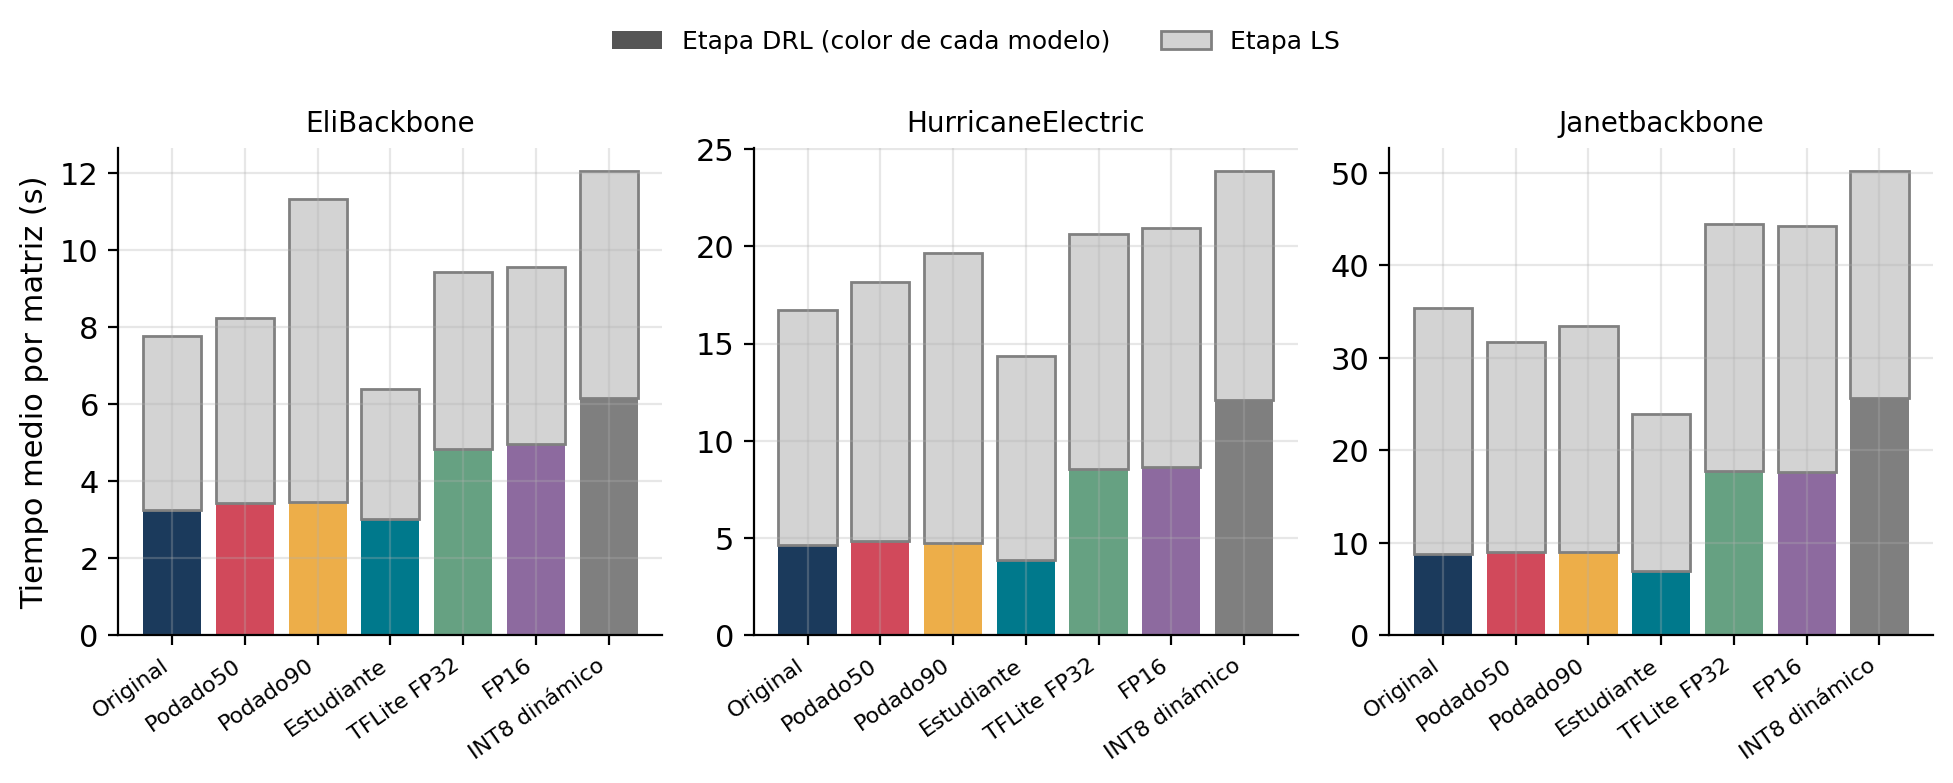
\includegraphics[width=\textwidth]{imagenes/fig_tiempos}
	\caption[Reparto del tiempo de optimización]{Tiempo medio de optimización de una matriz de tráfico, en segundos, repartido entre la etapa DRL y la LS, para cada modelo, en las tres topologías de evaluación. El estudiante es el de la semilla 9.}
	\label{fig:res_tiempos}
\end{figure}

Con los modelos de TensorFlow, la LS ocupa entre el 69 y el 73\,\% del tiempo total, y la etapa DRL, entre 4,6 y 5,8~s por matriz. Dentro de esta etapa, la inferencia de la red es solo una parte: la mayor parte del tiempo se dedica a construir los grafos de los candidatos y a simular la red en Python. Por ello, acelerar la red neuronal tiene un efecto limitado sobre el tiempo total.

El estudiante reduce el tiempo total entre un 5 y un 25\,\%. El 5\,\% se debe a su menor latencia, que reduce la etapa DRL de 5,6 a 4,6~s por matriz, y lo consigue cualquier estudiante. Cuando, además, proporciona a la LS un mejor punto de partida, como el de la semilla 9, esta necesita menos iteraciones para converger (27 frente a 43 en Janetbackbone, donde el tiempo total se reduce en torno a un tercio), y el ahorro medio en las tres topologías alcanza el 25\,\%.

\subsection{Impacto energético}

La Tabla~\ref{tab:res_energia} estima la energía de cada optimización con la Ecuación~\eqref{eq:energia}, como el producto de la potencia media del procesador medida durante el entrenamiento (23,9~W, Sección~\ref{sec:costes_energia}) por el tiempo de optimización de una matriz. Para dar una idea del consumo en operación, la extrapola a un año suponiendo una optimización cada 5 minutos.

\begin{table}[H]
	\centering
	\footnotesize
	\setlength{\tabcolsep}{4pt}
	\begin{adjustbox}{max width=\textwidth}
	\begin{tabular}{lccccc}
		\toprule
		& \textbf{Tiempo} & \textbf{Tiempo total} & \textbf{Energía por} & \textbf{Energía} & \textbf{Frente al} \\
		\textbf{Método} & \textbf{etapa DRL} & \textbf{por matriz} & \textbf{optimización} & \textbf{anual} & \textbf{original} \\
		\midrule
		Original & 5,56~s & 19,96~s & 477~J & 13,9~kWh & -- \\
		Podado50 & 5,78~s & 19,37~s & 463~J & 13,5~kWh & $-3$\,\% \\
		Podado90 & 5,75~s & 21,46~s & 513~J & 15,0~kWh & $+8$\,\% \\
		Estudiante (semilla 9) & 4,61~s & 14,89~s & 356~J & 10,4~kWh & $-25$\,\% \\
		TFLite FP32 & 10,39~s & 24,85~s & 594~J & 17,3~kWh & $+25$\,\% \\
		FP16 & 10,44~s & 24,94~s & 596~J & 17,4~kWh & $+25$\,\% \\
		INT8 dinámico & 14,64~s & 28,70~s & 686~J & 20,0~kWh & $+44$\,\% \\
		\bottomrule
	\end{tabular}
	\end{adjustbox}
	\caption[Energía estimada por optimización y anual]{Tiempo medio por matriz en las topologías de evaluación y energía estimada por optimización y por año (una optimización cada 5 minutos, $N_{\text{ejec}} = 105\,120$), con una potencia de 23,9~W.}
	\label{tab:res_energia}
\end{table}

Las cifras absolutas son pequeñas, porque corresponden a un único optimizador en un procesador de bajo consumo; lo relevante son las diferencias relativas, que se multiplican cuando el optimizador se ejecuta en muchos controladores o con mayor frecuencia. El estudiante es la única variante que reduce el consumo de forma apreciable, entre un 5 y un 25\,\% según la calidad del punto de partida que proporcione a la LS. La poda apenas modifica el consumo, y la cuantización con TensorFlow Lite lo aumenta en este procesador, porque alarga el tiempo de optimización. La estimación utiliza la potencia de la CPU bajo carga sostenida, por lo que es aproximada; la comparación entre modelos, que depende sobre todo de los tiempos medidos, es más fiable que los valores absolutos.

Estas cifras permiten también comparar la energía que se consume una sola vez con la que se ahorra en operación (Sección~\ref{sec:costes_energia}). El entrenamiento del agente base consumió unos 2,1~kWh en el procesador (23,9~W durante unas 87 horas). Con una optimización cada 5 minutos, el ahorro del estudiante igualaría esa energía en unos siete meses en el mejor caso (ahorro del 25\,\%) y en unos tres años en el peor (5\,\%). El coste que añade realmente la compresión es el de la destilación, que ocupa el equipo solo unas horas, por lo que se amortiza mucho antes.

% =====================================================================
\section{Comparación con la formulación exacta}\label{sec:res_milp}

Las secciones anteriores comparan cada modelo comprimido con el original, y muestran que la compresión reduce su coste sin empeorar el enrutamiento. Queda por responder una pregunta previa desde el punto de vista práctico: si ENERO, original o comprimido, es una buena forma de resolver este problema. Para ello se compara con las dos variantes de la formulación exacta MILP del enrutamiento por punto intermedio (Sección~\ref{sec:milp}), sobre las mismas matrices y en el mismo equipo. La Tabla~\ref{tab:res_milp} recoge la mejora sobre OSPF y el tiempo por matriz de cada método en las diez topologías, y la Figura~\ref{fig:res_calidad_tiempo} los representa de forma conjunta. De los modelos comprimidos se incluye el estudiante, que es el más rápido; el resto obtiene una calidad y unos tiempos similares a los del original (Secciones~\ref{sec:res_calidad} y~\ref{sec:res_energia}).

\begin{table}[H]
	\centering
	\footnotesize
	\setlength{\tabcolsep}{4pt}
	\begin{adjustbox}{max width=\textwidth}
	\begin{tabular}{lccccc}
		\toprule
		& \textbf{ENERO} & \textbf{ENERO} & \textbf{MILP} & \textbf{MILP} & \textbf{Cota} \\
		\textbf{Topología} & \textbf{original} & \textbf{estudiante} & \textbf{demandas críticas} & \textbf{todas las demandas} & \textbf{LP} \\
		\midrule
		EliBackbone & 41,3 (7,8) & 42,8 (6,4) & 41,5 (0,39) & 44,0 (9,5) & 44,1 \\
		HurricaneElectric & 34,5 (16,7) & 29,6 (14,4) & 41,2 (0,16) & 52,5 (9,8) & 52,7 \\
		Janetbackbone & 27,3 (35,4) & 40,6 (23,9) & 38,1 (0,31) & 51,0 (10,1) & 51,1 \\
		\textit{Media} & 34,3 (20,0) & 37,7 (14,9) & 40,3 (0,28) & 49,2 (9,8) & 49,3 \\
		\midrule
		WideJpn & 18,7 (42,1) & 18,9 (40,1) & 24,1 (0,20) & 36,8 (0,53) & 36,8 \\
		GtsPoland & 15,7 (32,8) & 15,0 (40,5) & 27,3 (4,3) & 35,1 (10,0) & 35,2 \\
		Bics & 25,1 (34,9) & 24,6 (31,1) & 26,6 (0,86) & 29,6 (8,7) & 29,6 \\
		Evolink & 9,4 (50,1) & 9,2 (47,2) & 10,8 (0,24) & 16,8 (2,2) & 16,8 \\
		Cesnet200511 & 19,9 (145,4) & 18,8 (141,1) & 37,0 (0,08) & 50,1 (4,8) & 50,3 \\
		LambdaNet & 11,1 (86,4) & 10,6 (86,5) & 15,2 (0,47) & 17,1 (8,8) & 17,1 \\
		Sanet & 13,7 (87,9) & 14,0 (91,6) & 15,2 (0,80) & 15,1 (10,1) & 15,2 \\
		\textit{Media} & 16,2 (68,5) & 15,9 (68,3) & 22,3 (0,99) & 28,7 (6,5) & 28,7 \\
		\bottomrule
	\end{tabular}
	\end{adjustbox}
	\caption[Comparación de ENERO con la formulación exacta MILP]{Mejora media de la MLU sobre OSPF (\%) y, entre paréntesis, tiempo medio por matriz (s) de ENERO completo (DRL + LS) con el modelo original y con el estudiante de la semilla 9, y de las dos variantes del MILP con un límite de 10~s, en las tres topologías de evaluación principales (50 matrices cada una) y en las siete redes mayores (10 matrices cada una). La última columna es la mejora máxima teórica que da la cota LP.}
	\label{tab:res_milp}
\end{table}

\begin{figure}[H]
	\centering
	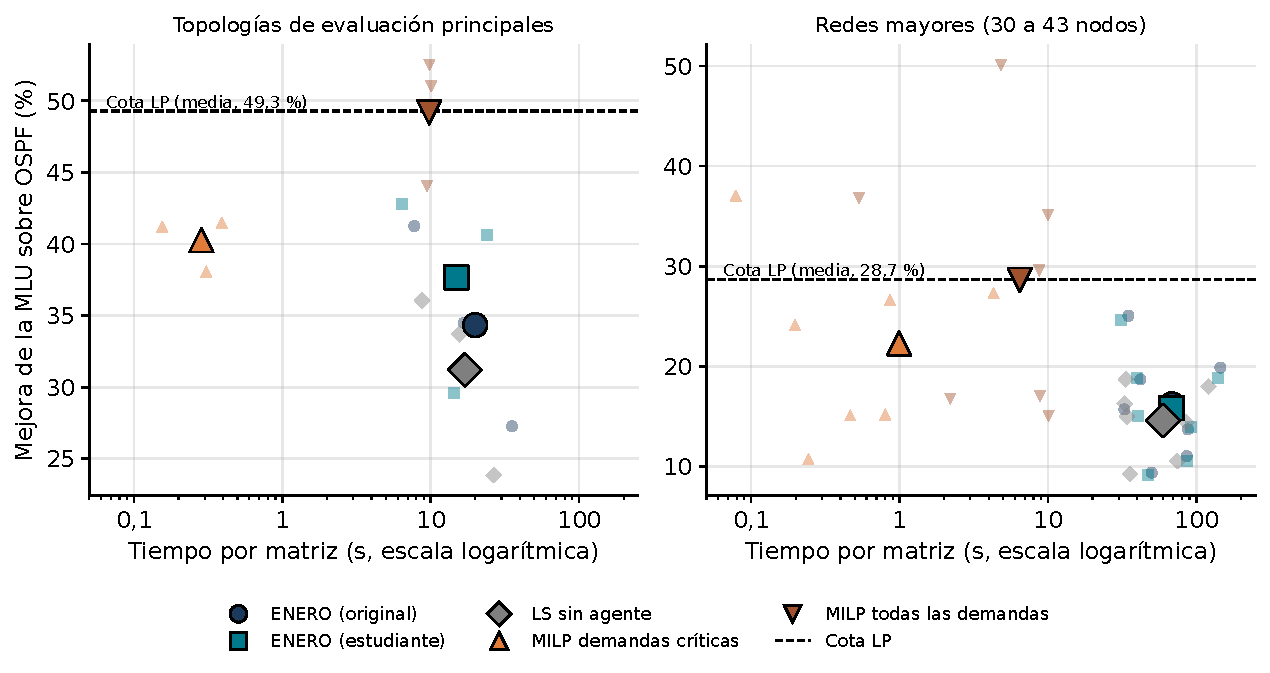
\includegraphics[width=\textwidth]{imagenes/fig_calidad_tiempo}
	\caption[Calidad frente a tiempo de optimización de cada método]{Mejora de la MLU sobre OSPF frente al tiempo por matriz, en escala logarítmica, de ENERO (modelo original y estudiante), la LS sin agente y las dos variantes del MILP. Los puntos pequeños corresponden a cada topología y los grandes, a la media de cada método. La línea discontinua marca la mejora media de la cota LP en cada grupo de redes.}
	\label{fig:res_calidad_tiempo}
\end{figure}

El primer resultado se refiere a la calidad. \textbf{El MILP sobre las demandas críticas mejora a ENERO original en las diez topologías}: un 40,3\,\% de media en las topologías principales y un 22,3\,\% en las redes mayores, frente al 34,3 y el 16,2\,\% de ENERO, que además aplica la LS. Como este MILP decide las mismas demandas que la etapa DRL, su resultado es el que obtendría el agente con una política perfecta, y la diferencia con ENERO mide cuánto se aleja de ese óptimo la política aprendida. Esa diferencia es pequeña en las redes parecidas a las de entrenamiento, como EliBackbone o Bics, y muy grande en las demás: en Cesnet200511, el MILP mejora a OSPF un 37,0\,\% y ENERO, un 19,9\,\%. Es la misma pauta de generalización observada en la Sección~\ref{sec:res_mayores}, ahora medida frente a un óptimo y no frente a la LS. El estudiante de la semilla 9 es el único modelo que supera a este MILP, en EliBackbone y Janetbackbone. Es posible porque la LS vuelve a seleccionar las demandas críticas a partir de la configuración que entrega la etapa DRL, de modo que puede modificar demandas que el MILP mantiene en su camino de OSPF.

El MILP sobre todas las demandas obtiene un 49,2\,\% de mejora media en las topologías principales y un 28,7\,\% en las mayores, prácticamente lo mismo que la cota LP (49,3 y 28,7\,\%). En todas las redes queda a menos de un 0,4\,\% de ella. Por tanto, en estas redes la restricción de un único nodo intermedio por demanda apenas limita la calidad, como apuntaban los resultados previos sobre el enrutamiento por segmentos \cite{bhatia2015optimized}, y casi toda la distancia entre ENERO y la cota LP (Sección~\ref{sec:res_generalizacion}) se debe al método de optimización y no al esquema de enrutamiento.

El segundo resultado se refiere al tiempo. \textbf{El MILP sobre las demandas críticas tarda de media 0,28~s por matriz en las topologías principales y 0,99~s en las redes mayores, unas 70 veces menos que ENERO} (20,0 y 68,5~s). Con el límite de 10~s, alcanzó el óptimo demostrado en 67 de las 70 matrices de las redes mayores; las tres restantes, en GtsPoland, quedaron a menos de un 0,2\,\% de la cota inferior que da el \textit{solver}, y con 60~s también se resolvieron de forma óptima. El MILP sobre todas las demandas tiene unas siete veces más variables y tarda más, 9,8 y 6,5~s de media, pero sigue siendo más rápido que ENERO en todas las redes salvo EliBackbone, la más pequeña. En las redes mayores agota el límite de 10~s en 37 de las 70 matrices; aun así, sus soluciones quedan a menos de un 0,5\,\% de la cota inferior, y con 60~s alcanza el óptimo en 60 de ellas, con 18,8~s de media. Este comportamiento es una ventaja práctica del método exacto: aunque se detenga antes de terminar, entrega una solución válida e indica cuánto puede alejarse del óptimo, algo que ENERO no proporciona. Como el tiempo del MILP no incluye la construcción del modelo en Python (Sección~\ref{sec:milp}), la comparación favorece algo al método exacto, pero la diferencia con ENERO es de casi dos órdenes de magnitud. Tampoco la compresión la reduce de forma apreciable: el estudiante, el modelo más rápido, sigue tardando entre 50 y 70 veces más que el MILP sobre las demandas críticas, y obtiene peor resultado que él en ocho de las diez redes.

El tercer resultado se refiere al coste de puesta en marcha y a la aplicabilidad. ENERO necesita un entrenamiento previo de unas 87 horas en CPU, a lo que se suma el de la compresión, y su calidad depende de que la red se parezca a las de entrenamiento: para desplegarlo en un tipo de red distinto habría que volver a entrenarlo o ajustarlo. El MILP no necesita entrenamiento; se construye a partir de la topología y de la matriz de tráfico de cada momento, por lo que se aplica igual a cualquier red y se adapta de forma inmediata a cambios en la topología. La diferencia también se refleja en la energía. Con el mismo modelo de la Sección~\ref{sec:res_energia}, una optimización con el MILP sobre las demandas críticas consume unos 7~J en las topologías principales, frente a los 477~J de ENERO original y los 356~J del estudiante, lo que supone unos 0,2~kWh al año frente a 13,9 y 10,4~kWh. Solo la energía del entrenamiento del agente base (unos 2,1~kWh) bastaría para más de diez años de optimizaciones con el MILP. La cifra es orientativa, porque la potencia del procesador durante la resolución puede diferir de la medida en el entrenamiento, pero la diferencia es lo bastante grande para no depender de ese detalle.

La ventaja del método exacto tiene un límite. El número de variables del MILP crece con el número de demandas y de candidatos, y el tiempo de resolución de un problema entero puede crecer de forma exponencial con su tamaño (Sección~\ref{sec:prog_mat}). Ese crecimiento ya se aprecia en la variante de todas las demandas, que agota el límite de 10~s en parte de las matrices de cinco de las siete redes mayores. Las redes evaluadas tienen como máximo 43 nodos, así que este trabajo no permite afirmar a partir de qué tamaño el MILP dejaría de resolverse en un tiempo razonable, que es donde un agente entrenado podría resultar competitivo.

En conjunto, \textbf{en las redes evaluadas, la formulación exacta es preferible a ENERO, original o comprimido, en calidad, en tiempo por optimización y en coste de puesta en marcha}. La compresión cumple su objetivo, ya que reduce el coste del agente sin empeorar el enrutamiento, pero no cambia esta comparación, porque la desventaja de ENERO no está en el tamaño de la red neuronal, sino en el propio enfoque de aprendizaje.

% =====================================================================
\section{Síntesis de resultados y recomendaciones}\label{sec:res_sintesis}

La Tabla~\ref{tab:res_sintesis} resume los efectos de cada técnica frente al modelo original en las topologías de evaluación principales.

\begin{table}[H]
	\centering
	\footnotesize
	\setlength{\tabcolsep}{4pt}
	\begin{adjustbox}{max width=\textwidth}
	\begin{tabular}{l>{\raggedright\arraybackslash}p{2.9cm}>{\raggedright\arraybackslash}p{2.1cm}>{\raggedright\arraybackslash}p{3.0cm}>{\raggedright\arraybackslash}p{1.6cm}}
		\toprule
		& \textbf{Tamaño} & \textbf{Latencia} & \textbf{Calidad (DRL + LS)} & \textbf{Energía} \\
		\midrule
		Podado50 & $-38$\,\% (gzip) & Sin cambio & Sin diferencias significativas & $-3$\,\% \\
		Podado90 & $-78$\,\% (gzip) & Sin cambio & Ligeramente peor, diferencia significativa ($-1{,}7$ puntos) & $+8$\,\% \\
		FP16 & $-25$\,\% (frente a TFLite FP32) & 4,5 veces mayor & Sin diferencias significativas & $+25$\,\% \\
		INT8 dinámico & $-40$\,\% (frente a TFLite FP32) & 7,6 veces mayor & Sin diferencias significativas & $+44$\,\% \\
		Estudiante & $-78$\,\% de parámetros & 3,2 veces menor & Similar en media & $-5$ a $-25$\,\% \\
		\bottomrule
	\end{tabular}
	\end{adjustbox}
	\caption{Síntesis de los efectos de cada técnica de compresión frente al modelo original.}
	\label{tab:res_sintesis}
\end{table}

La destilación es la técnica que mejor se adapta a este problema: es la única que reduce la latencia en un procesador de propósito general, porque modifica la arquitectura y no solo la representación de los pesos, y conserva en media la calidad del original, también en redes mayores. Su principal limitación es que el resultado de un estudiante concreto varía con el entrenamiento, por lo que conviene validarlo antes de desplegarlo. La poda moderada reduce el almacenamiento sin pérdida de calidad, pero sus beneficios en tiempo requerirían hardware capaz de aprovechar los ceros. La cuantización reduce el tamaño del fichero, pero en un modelo tan pequeño la ganancia es limitada y, con TensorFlow Lite, aumenta el tiempo de ejecución en este procesador.

En función del tipo de red, los resultados permiten orientar la elección:
\begin{itemize}
	\item \textbf{En redes parecidas a las de entrenamiento} (grado medio en torno a 3 y tamaño similar), el agente mejora claramente a la LS y su compresión resulta útil: con poda moderada si la restricción es el almacenamiento, o con destilación si lo es la latencia.
	\item \textbf{En redes mayores o más dispersas}, todos los modelos comprimidos rinden como el original, pero el agente aporta menos sobre la LS. Antes de comprimirlo convendría entrenarlo con topologías de ese tipo.
	\item \textbf{Si la restricción es el almacenamiento o la distribución del modelo}, el estudiante es la opción más compacta sin pérdida de calidad (9,9~KB comprimido), seguido de INT8 dinámico y de la poda al 50\,\% (27,7 y 28,3~KB).
\end{itemize}

Estas recomendaciones indican cómo comprimir el agente si se opta por ENERO. Sin embargo, al valorar los métodos no solo por la calidad del enrutamiento, sino también por su aplicabilidad práctica, la conclusión es otra: \textbf{en redes de hasta unas decenas de nodos, como las evaluadas, la metodología más adecuada es la formulación exacta (Sección~\ref{sec:res_milp}). El MILP sobre las demandas críticas es la opción más práctica, porque resuelve de forma óptima el problema de la etapa DRL en menos de un segundo y sin entrenamiento previo; el MILP sobre todas las demandas es preferible si prima la calidad, ya que alcanza prácticamente la cota LP en unos segundos. ENERO y sus versiones comprimidas solo podrían tener interés en redes mucho mayores, en las que el método exacto deje de resolverse en un tiempo razonable.}
